\chapter{Experimental Results}

In this chapter we present our obtained data and their analysis of the measurements from oscillatory experiments as introduced in \textbf{Experimental Approach} chapter.

In the first part, we present our drag force measurements by using all three oscillators submerged in superfluid Helium-II in hydrodynamical regime at temperatures $T > 1 \unit{K}$).

Next, we add measurements from the ballistic regime at temperatures $T < 0.6 \unit{K}$ abd connect them in order to prove the concept of universal scaling.

As the last analysis we introduce a \textit{flow phase diagram}, summarizing all our foundings basically in a single graph, representing the areas of different non-linear regimes.

\newpage

\section{Drag force measurements}

As we introduced in the last section of \textbf{Experimental approach} chapter, we used the full frequency sweep method for vibrating wire and tuning fork. Each point on following graphs was obtained by a pair of full frequency sweeps across the resonance of given oscillator. One sweep was performed with increasing frequency and the second one with decreasing frequency, which made us confident that no hysteresis effect was present.

We present all the measurements in the form of typical hydrodynamic visualizations (velocity-force response, drag coefficients and appropriate dimensionless numbers) of oscillating wire, torsional disc and tuning fork, respectively.

\subsection{Vibrating NbTi wire}

We were measuring both the voltage in-phase with the driving current and the quadrature signal, in order to obtain the resonant response. When a high enough applied drives were reached ($\gtrsim 0.8 \unit{mA}$ at temperature $1.67\unit{K}$, responding in $\sim 0.1 \unit{m/s}$ peak velocity), there was present a resonant frequency shift and a \textit{peak softening} effect.\\
As the calibration of the magnetic field produced by permanent magnets was performed only at room temperature, the peak velocity on the wire top is known with the accuracy about $\pm 20 \%$. This error doesn't affect the scaling process obtained from the data.

\begin{figure}[h]
	\centering
	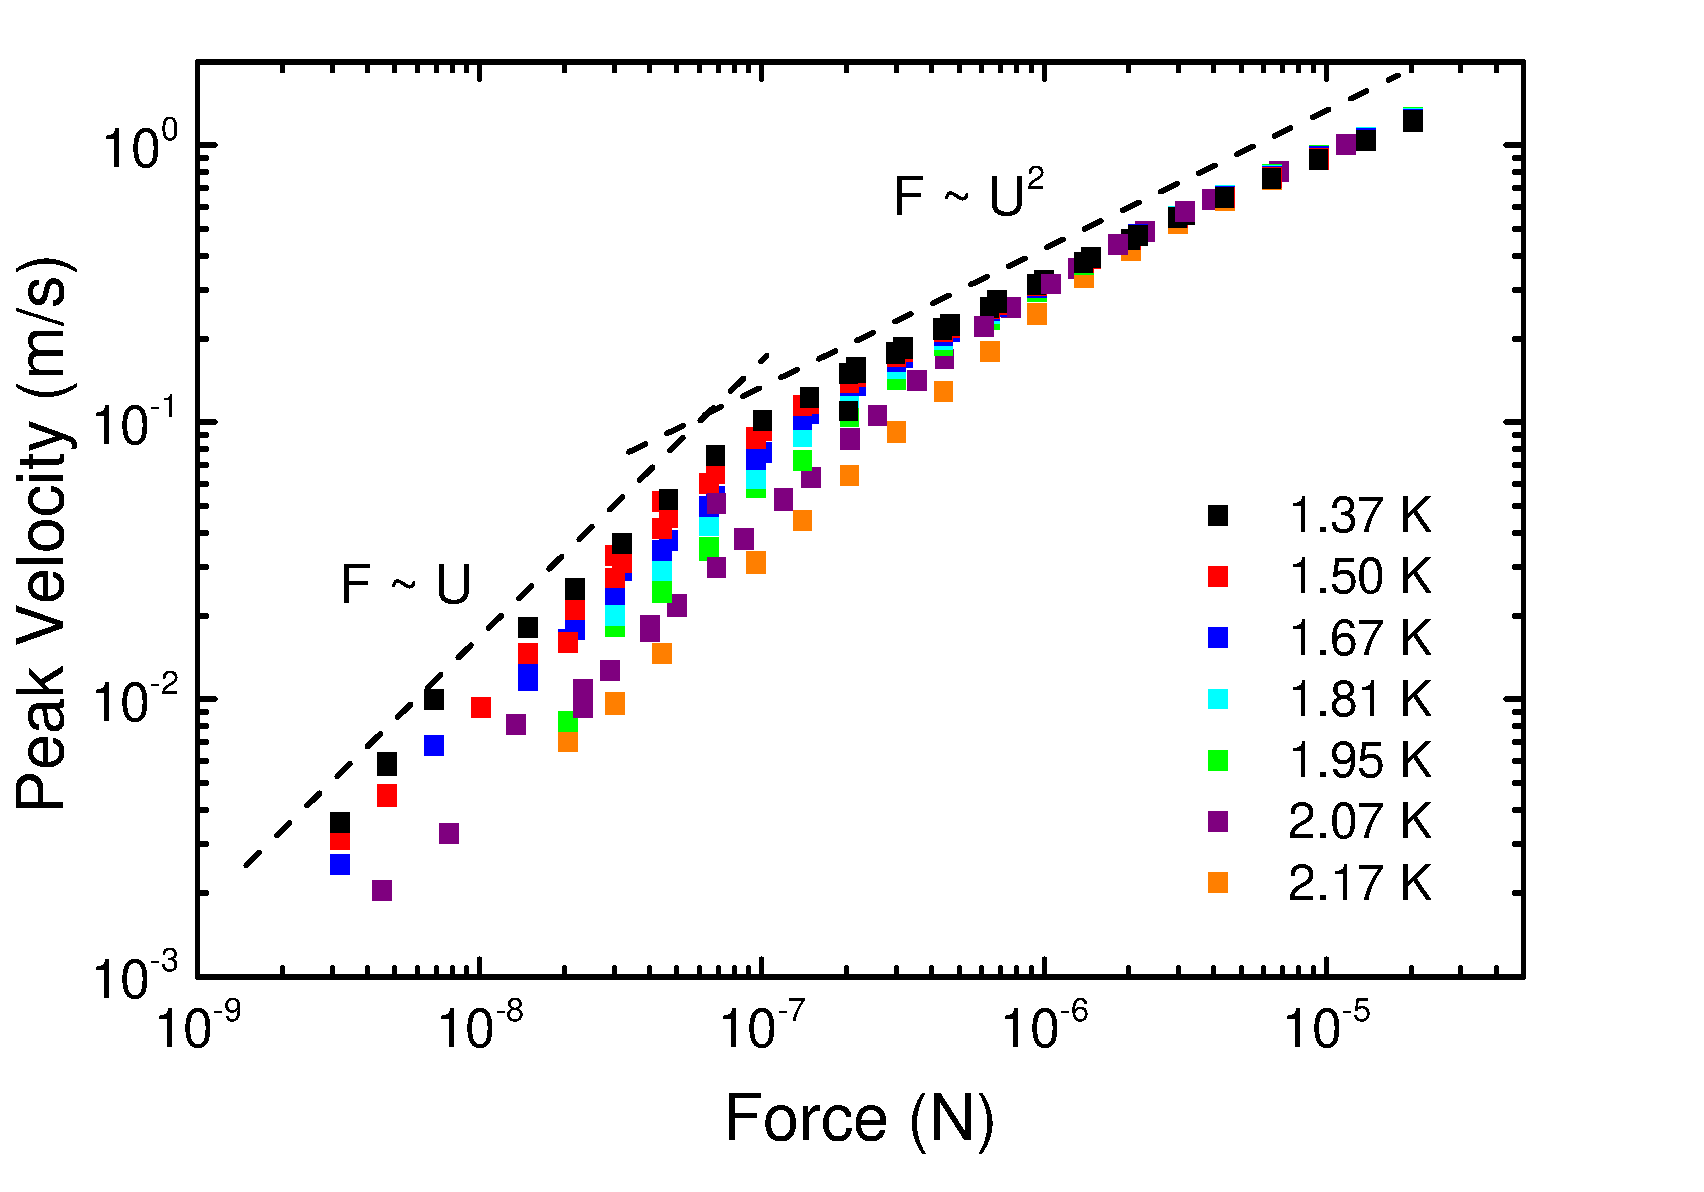
\includegraphics[width=0.7\textwidth]{graphics/results/wire_force_vel}
	\caption{Plot of peak velocity $U_0$ against the applied peak force $F_0$ for the vibrating wire submerged in superfluid $\He$ at several temperatures. The \underline{black dashed lines} serve as sketch of theoretical laminar and turbulent regimes.}
	\label{wire_vel_force}
\end{figure}

We plot in \textbf{Figure \ref{wire_vel_force}} the peak velocity of the wire top $U_0$ against the applied peak force $F_0$ at various temperatures from two-fluid regime ($T > 1.0\unit{K}$).

Clearly, the wire exhibits linear drag at low velocities and non-linear additional drag in the area of higher velocities. The energy losses of the wire in the low-velocity part are dominated by the viscous drag of the present normal component. Other loss mechanisms like acoustic emission are in principle present as well, but neglected in further discussion. The additional dissipation process in the higher-velocity part indicates either classical or quantum turbulence (or both) and the measured drag $F_0$ is roughly proportional to $U_0^2$.

Next we plot in \textbf{Figure \ref{wire_drag_vel}} the classical drag coefficient as a function of peak force and velocity $C_D \sim F_0 / U_0^2$ using the same data as presented in \textbf{Figure \ref{wire_vel_force}}.

\begin{figure}[h]
	\centering
	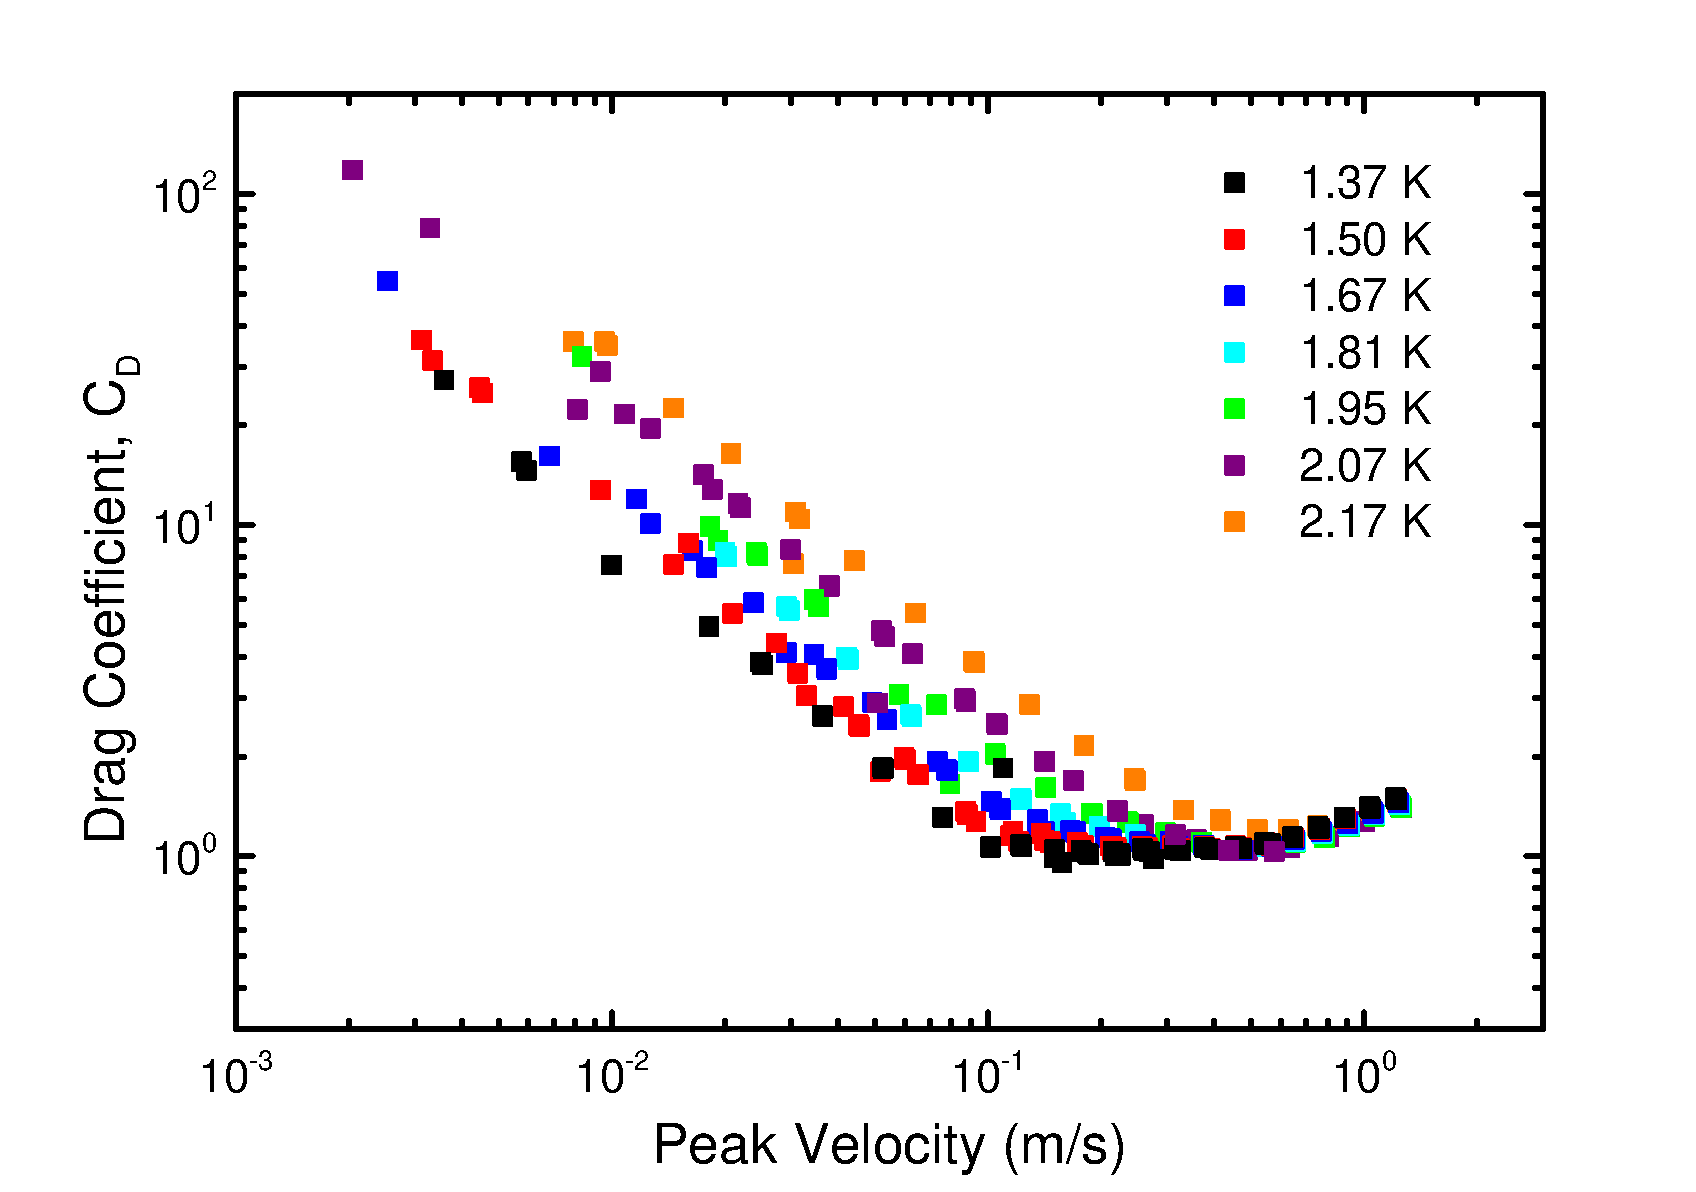
\includegraphics[width=0.7\textwidth]{graphics/results/wire_drag_vel}
	\caption{Plot of drag coefficient $C_D$ against the velocity peak response $U_0$ for the vibrating wire at several temperatures.}
	\label{wire_drag_vel}
\end{figure}

In order to perform the universal scaling, we collapse the contribution of the normal component in the following way:

\begin{equation}
C_D^{\,n} \leftarrow C_D \frac{\rho}{\rho_n}\,,
\hspace{1cm}
\text{Dn} \leftarrow U_0 \sqrt{\frac{2\rho_n}{\eta\omega}}\,,
\label{universal_scale}
\end{equation}

where $\eta$ is the dynamical viscosity of Helium-II for a given temperature. Relations in (\ref{universal_scale}) are applied in the same way as described (\ref{drag_normal}), (\ref{donnelly}) in the last section of \textbf{Theoretical background} chapter.\\
The resulting plot \textbf{Figure \ref{wire_drag_donnelly}} clearly shows the collapse of all linear parts of the measured drag into a single line. However, the theoretical pre-factor ($\Phi_{\text{cyl}} = 4\pi$) is smaller than the fitted one ($\Phi \sim 26$). This cannot be explained by experimental errors such as the magnet calibration, so the most likely reason behind it is the effect of irregularities on the surface of the wire. Indeed, excrescences of order $5 \mu\text{m}$ were observed on the $40 \mu \text{m}$ wire under an optical microscope.


\begin{figure}[h]
	\centering
	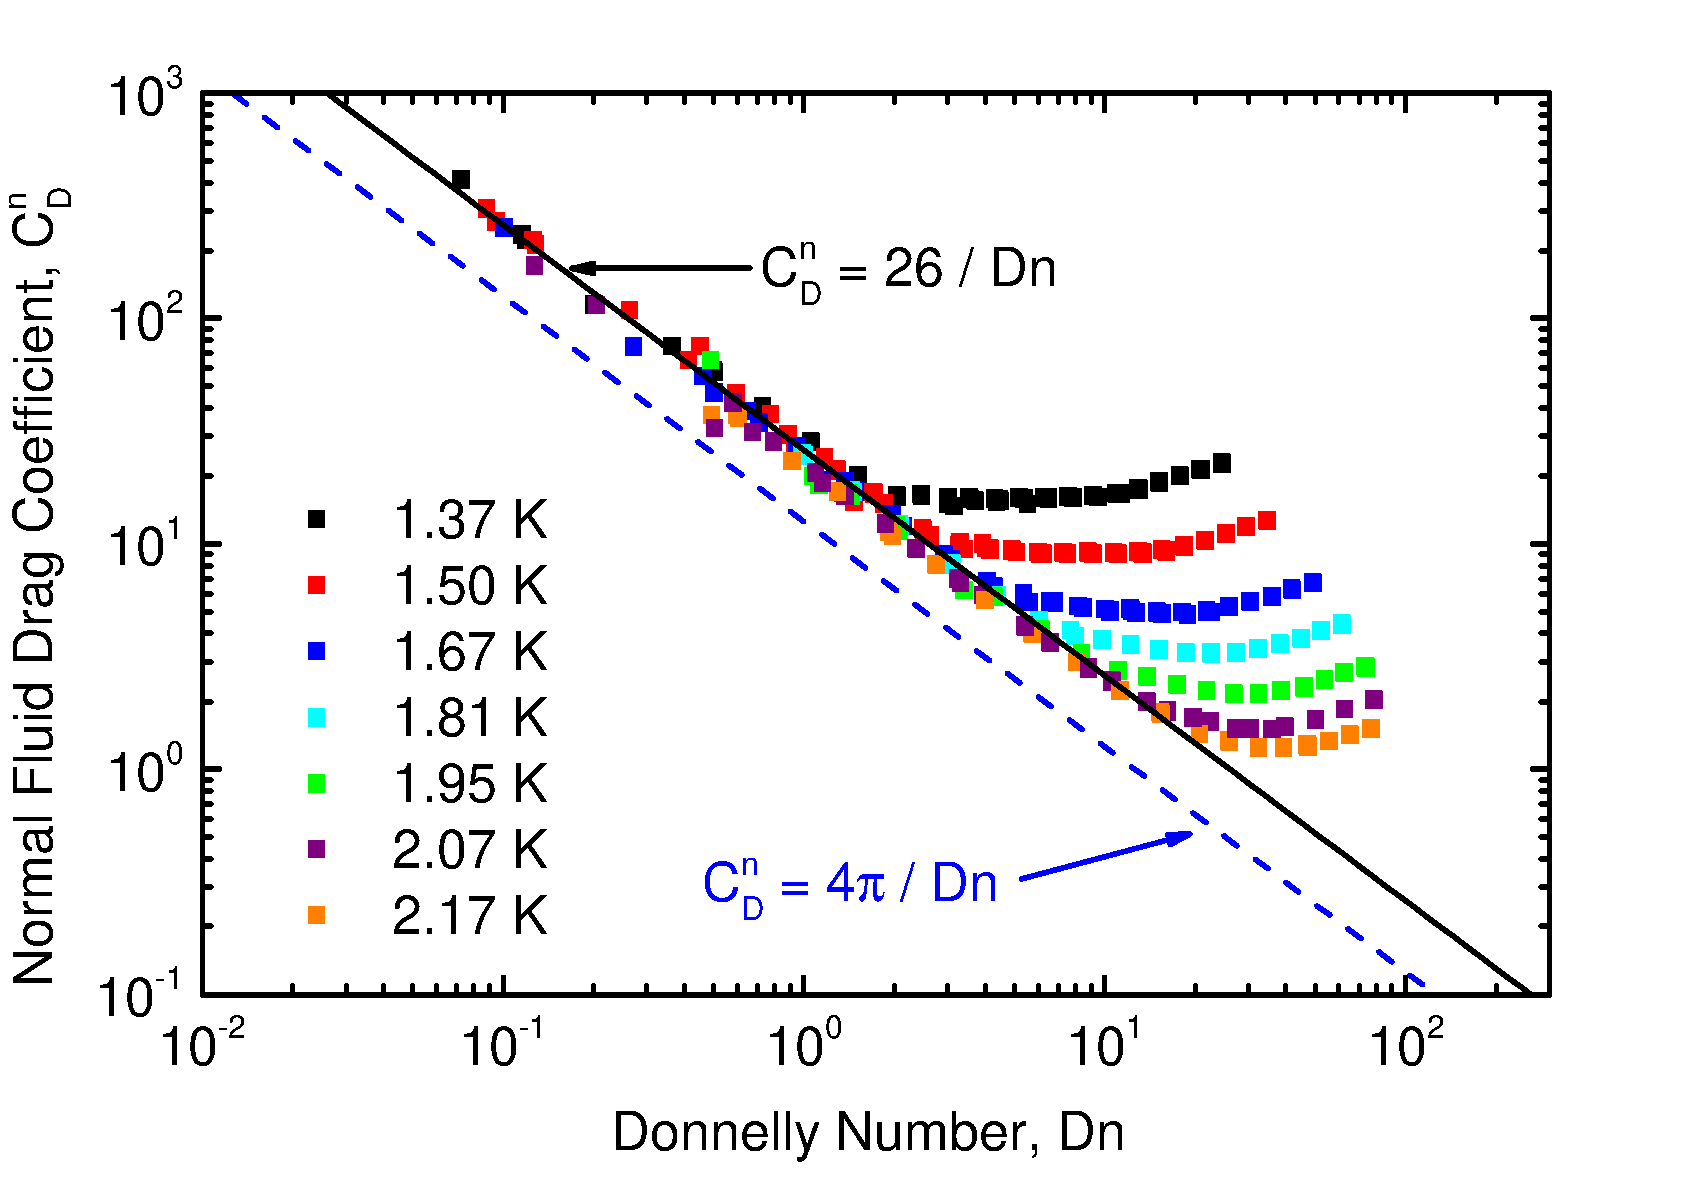
\includegraphics[width=0.7\textwidth]{graphics/results/wire_drag_donnelly}
	\caption{Plot of normal fluid drag coefficient $C_D^{\,n}$ against the dimensionless Donnelly number (Dn) for the vibrating wire at several temperatures.The \underline{blue dashed line} shows the expected theoretical dependence \cite{universal_scaling} for a smooth cylinder. The \underline{solid black line} is a numerical fit of the linear part of data.}
	\label{wire_drag_donnelly}
\end{figure}

One may see from the \textbf{Figure \ref{wire_drag_donnelly}} that all temperature curves are visually sorted ascendingly as the non-linear behaviour occurs at certain starting points. These points of non-linearity emergence cannot be governed by a single value of Donnelly number, but rather with a critical veloicity $U_C$.

We show in \textbf{Figure \ref{wire_nonlinear_drag}} that all deviations can be connected by the exceeding of critical dimensionless velocity $\hat{U}_C = U_C / \sqrt{\varkappa \omega}$. The approximate value of the critical $\hat{U}_C$ was found using \textit{error plot}, where the \textit{error} is defined via the absolutized errors of linear superfluid drag coefficient function $C_D^{\, s} = C_D \rho / \rho_s = \gamma / \hat{U}$:

\begin{equation}
\text{Error} = \frac{\text{abs}(C_D^{\,s} \hat{U} - \gamma)}{C_D^{\,s} \hat{U}} \in (0,1)\,,
\end{equation}

where $\gamma$ is the pre-factor coefficient, different for each temperature curve.

The single critical value $\hat{U}_C \sim 1$ (see \textbf{Figure \ref{wire_nonlinear_drag}}) is thus a clear sign of the onset of quantum turbulence by the superfluid component.

\begin{figure}[h]
	\centering
	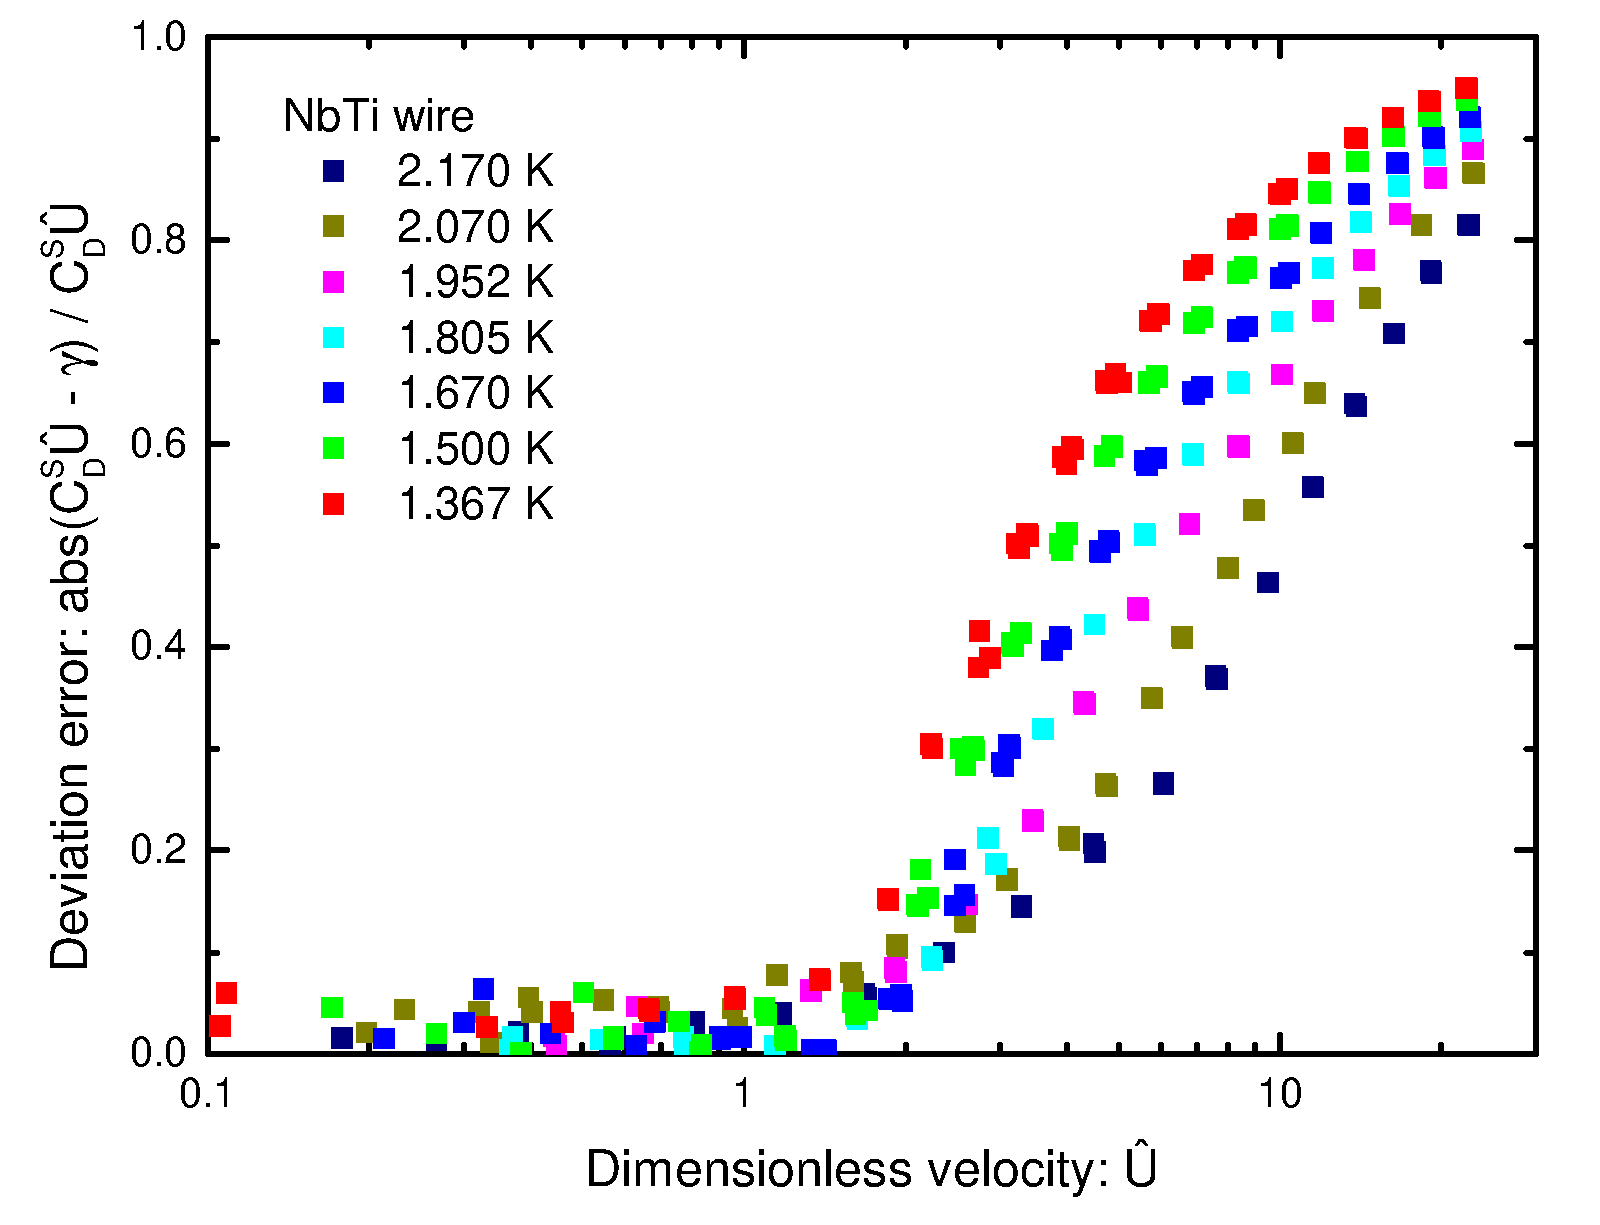
\includegraphics[width=0.7\textwidth]{graphics/results/wire_nonlinear_drag}
	\caption{Plot of normalized deviations from the linear fits $C_D^{\,s} =  \gamma / \hat{U}$ with $\gamma$ differing for each curve, as a function of the dimensionless velocity $\hat{U}$ for various temperatures from the studied range.}
	\label{wire_nonlinear_drag}
\end{figure}


%%%%%%%%%%%%%%%%%%%%%%%%%%%%%%%%%%%%%%%%%%%%%%%%%%%%%%%%%%%%%%%%%%%%%%%%%%%%%%%%%%%%%%%

\subsection{Oscillating disc}

The (torsionally) oscillating disc differs from the vibrating wire in several technicalities:

\begin{itemize}
  \item Oscillating disc does not displace any fluid and thus The superfluid is at rest unless quantized vorticity is produced
  \item It is not possible to perform measurements in a steady state of flow, but decayed flow was measured instead
  \item Drag force has to be inferred from the decaying amplitude of oscillator deflection.
\end{itemize}

As a consequence of mentioned differences (examples showed in \textbf{Figure \ref{disc_extrema}}), we have to substitute $U_0 = \omega R \phi_0$ within the Donnelly number and define a new drag coefficient, specific for our mechanical system of torsionally oscillating disc in a viscous fluid of density $\rho_n$ as:
\begin{equation}
C_D^{\,n} \leftarrow \frac{2M_f}{A\rho_n \Omega_0^2 R^3}\,,
\hspace{1cm}
\text{Dn} \leftarrow R\omega \phi_0 \sqrt{\frac{2\rho_n}{\eta\omega}}\,,
\label{disc_scale}
\end{equation}

where $M_f$ is the moment of friction forces, $R$ the radius of the disc, $A = \pi R^2$ the area of the disc and $\Omega_0$ is the amplitude of angular frequency $\omega(t)$. It was already showed \cite{universal_scaling} the relation between such drag coefficient (\ref{disc_scale}) can be expressed in laminar flow in terms of the Donnelly number as $C_D^{\,n} = \Phi /\text{Dn}$ with the pre-factor $\Phi_{\text{disc}} = 2$.

\begin{figure}[h]
	\centering
  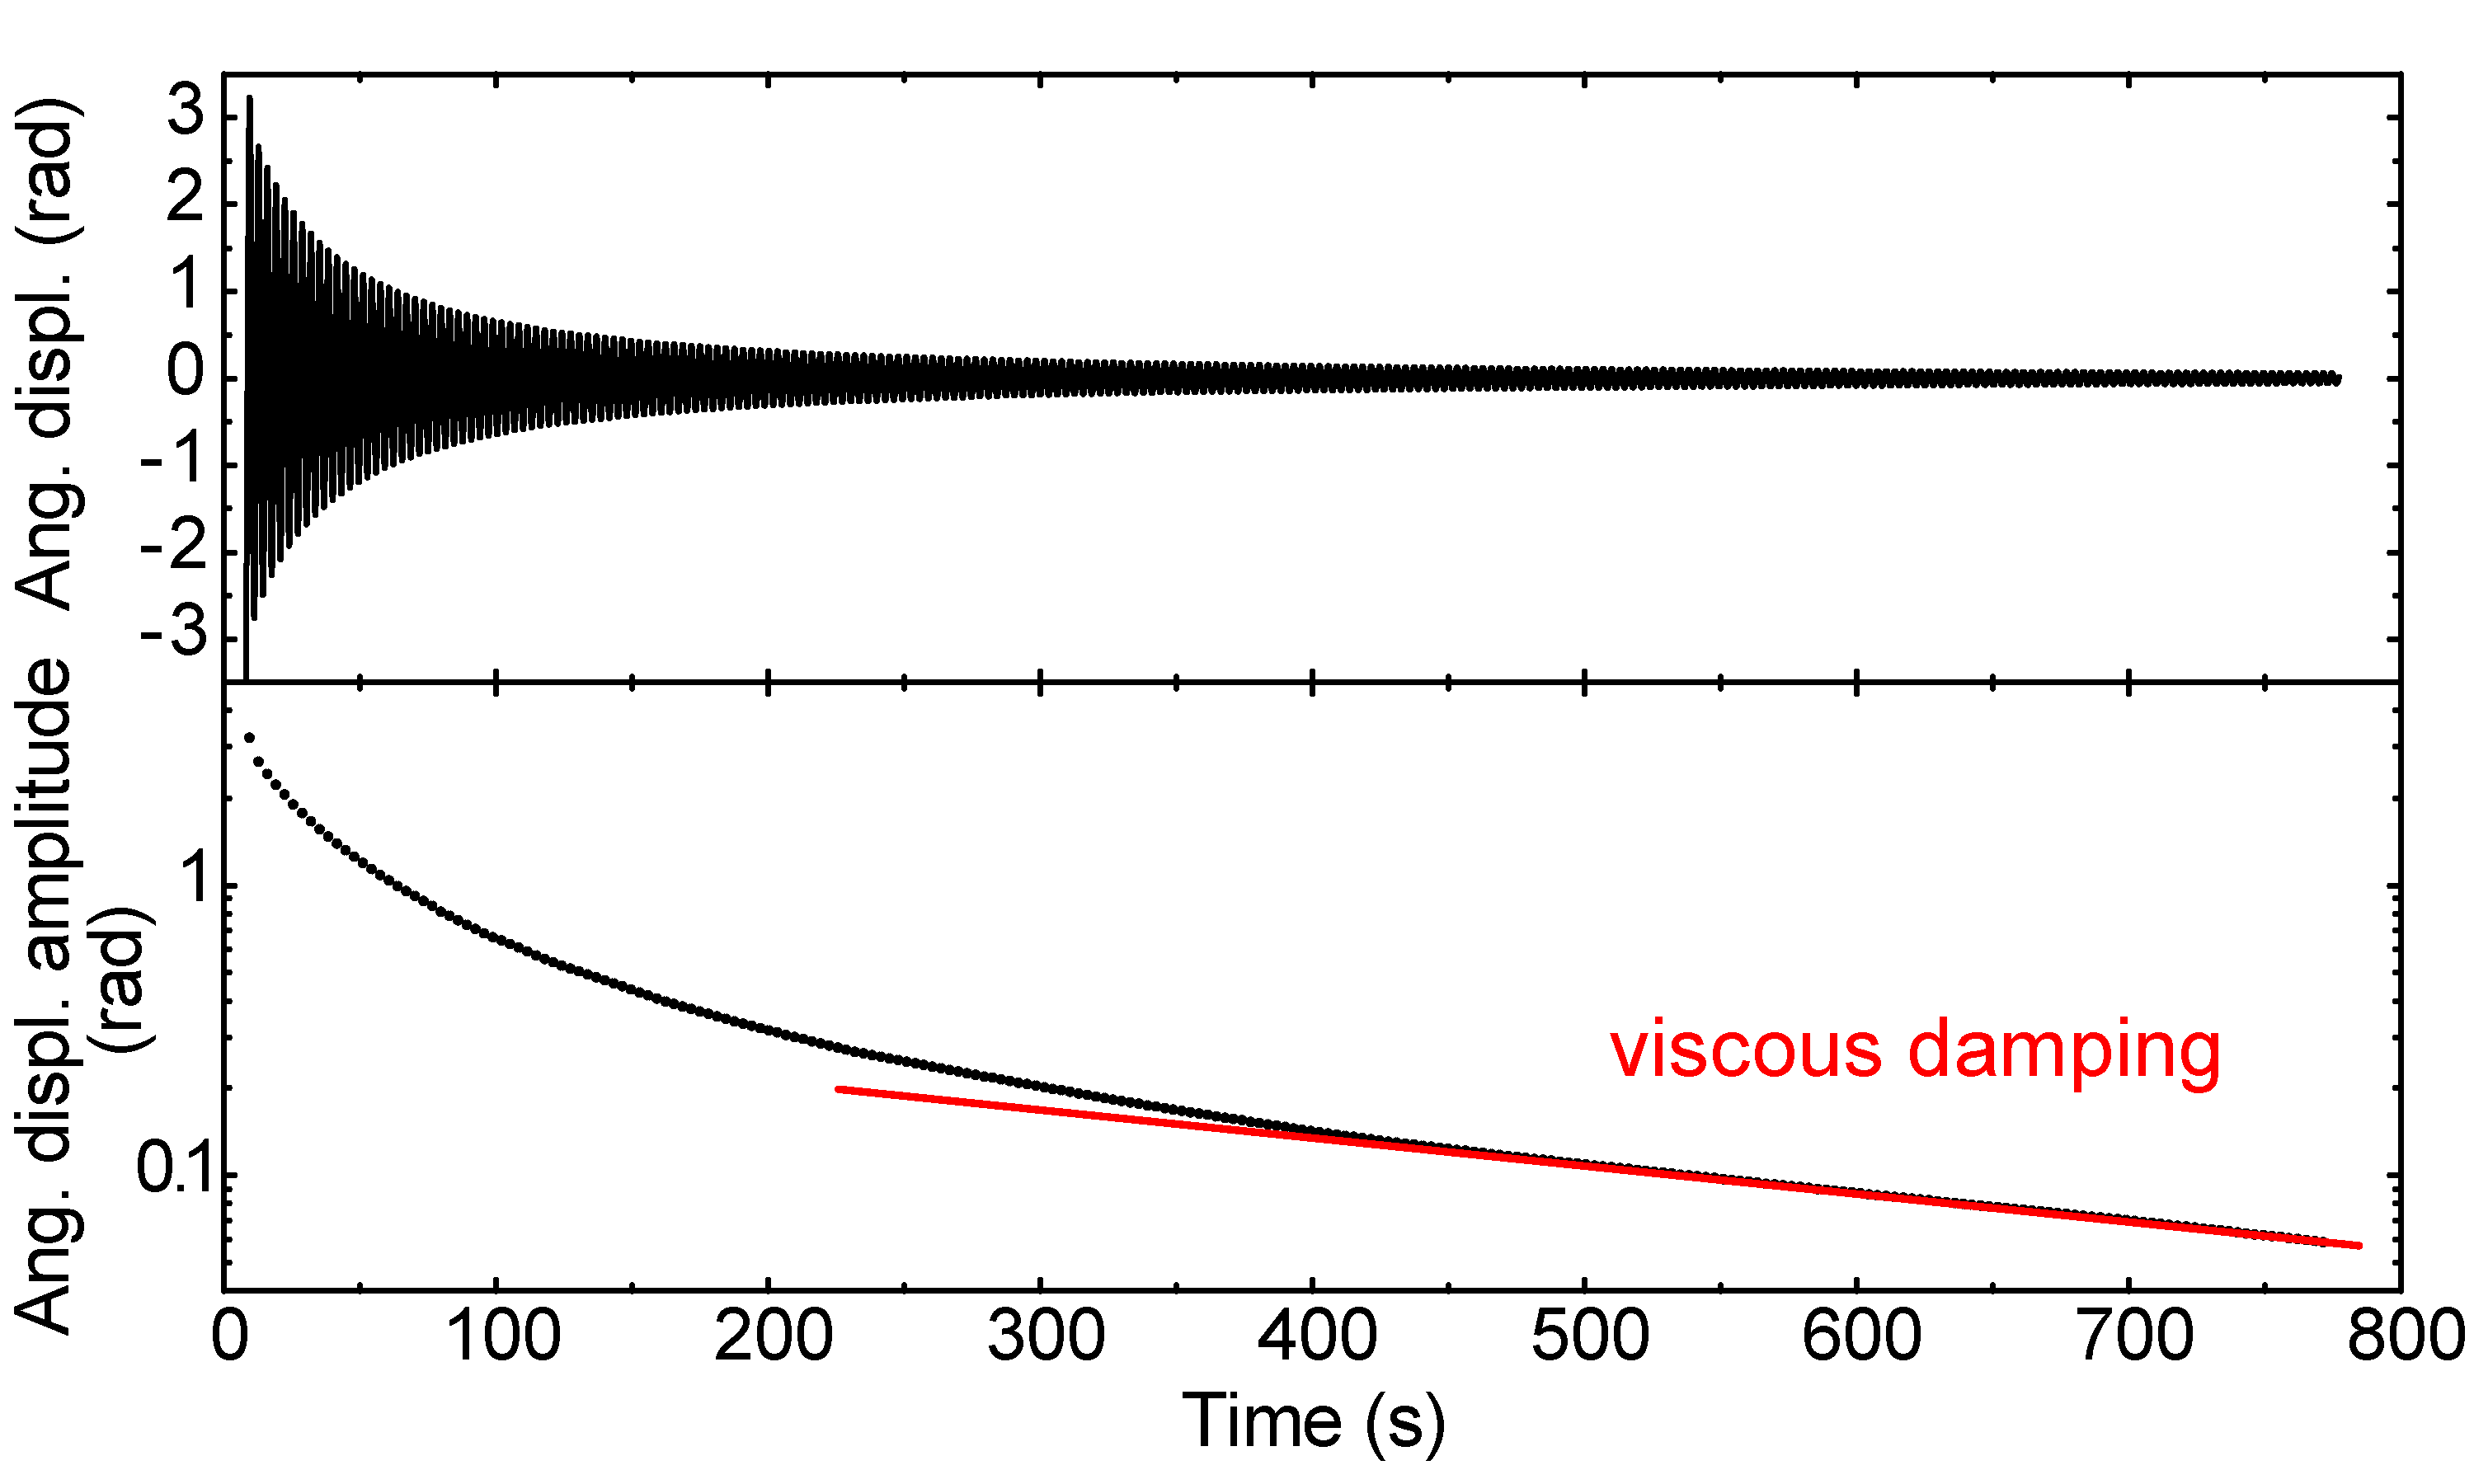
\includegraphics[width=0.8\textwidth]{graphics/results/disc_extrema}
  \caption{Example of angular displacement measurement in time of the torsionally oscillating disc.\\
  \underline{Top picture:} The decreasing angular displacement amplitudes $\phi_0 (t)$.
  \underline{Bottom picture:} The logarithmic plot $\phi_0 (t)$ shows two distinct regions – nonlinear decay in the area of earlier times $t < 400$ due to turbulent drag forces and an exponential (viscous) decay due to laminar flow of the normal component at the later times $t > 500$.}
  \label{disc_extrema}
\end{figure}

We plot the re-defined drag coefficient $C_D^{\,n}$ (\ref{disc_scale}) against the Donnelly number in \textbf{Figure \ref{disc_drag_donnelly}}.
Again, as in case of vibratig wire, the data collapse to a single inverse dependence $C_D^{\,n} = 2 / \text{Dn}$ in the area of small values of Donnelly number, which illustrates and proves the universal scaling concept.\\
One would naturally expect the normal component to transit to turbulent regime earlier than the superfluid one since the oscillating disc directly moves only with the normal component. However, \textbf{Figure \ref{disc_drag_donnelly}} clearly shows that non-linearities are not characterized by a single value of Dn, but rather continuously with ascending temperature. This implies that instabilities cannot be explained by pure viscous fluid dynamics and must relate to the quantum turbulence produced by a Donnelly-Glaberson instability.

We don't provide the error plot for this oscillator since it looks practically identical to the one presented with vibrating wire and brings no additional information. The critical dimensionless velocity of the torsionally oscillating disc is estimated (from the error plot) as $\hat{U}_C \sim 12$. This is about one order higher than in the case of vibrating wire.

\newpage

\begin{figure}[h]
	\centering
  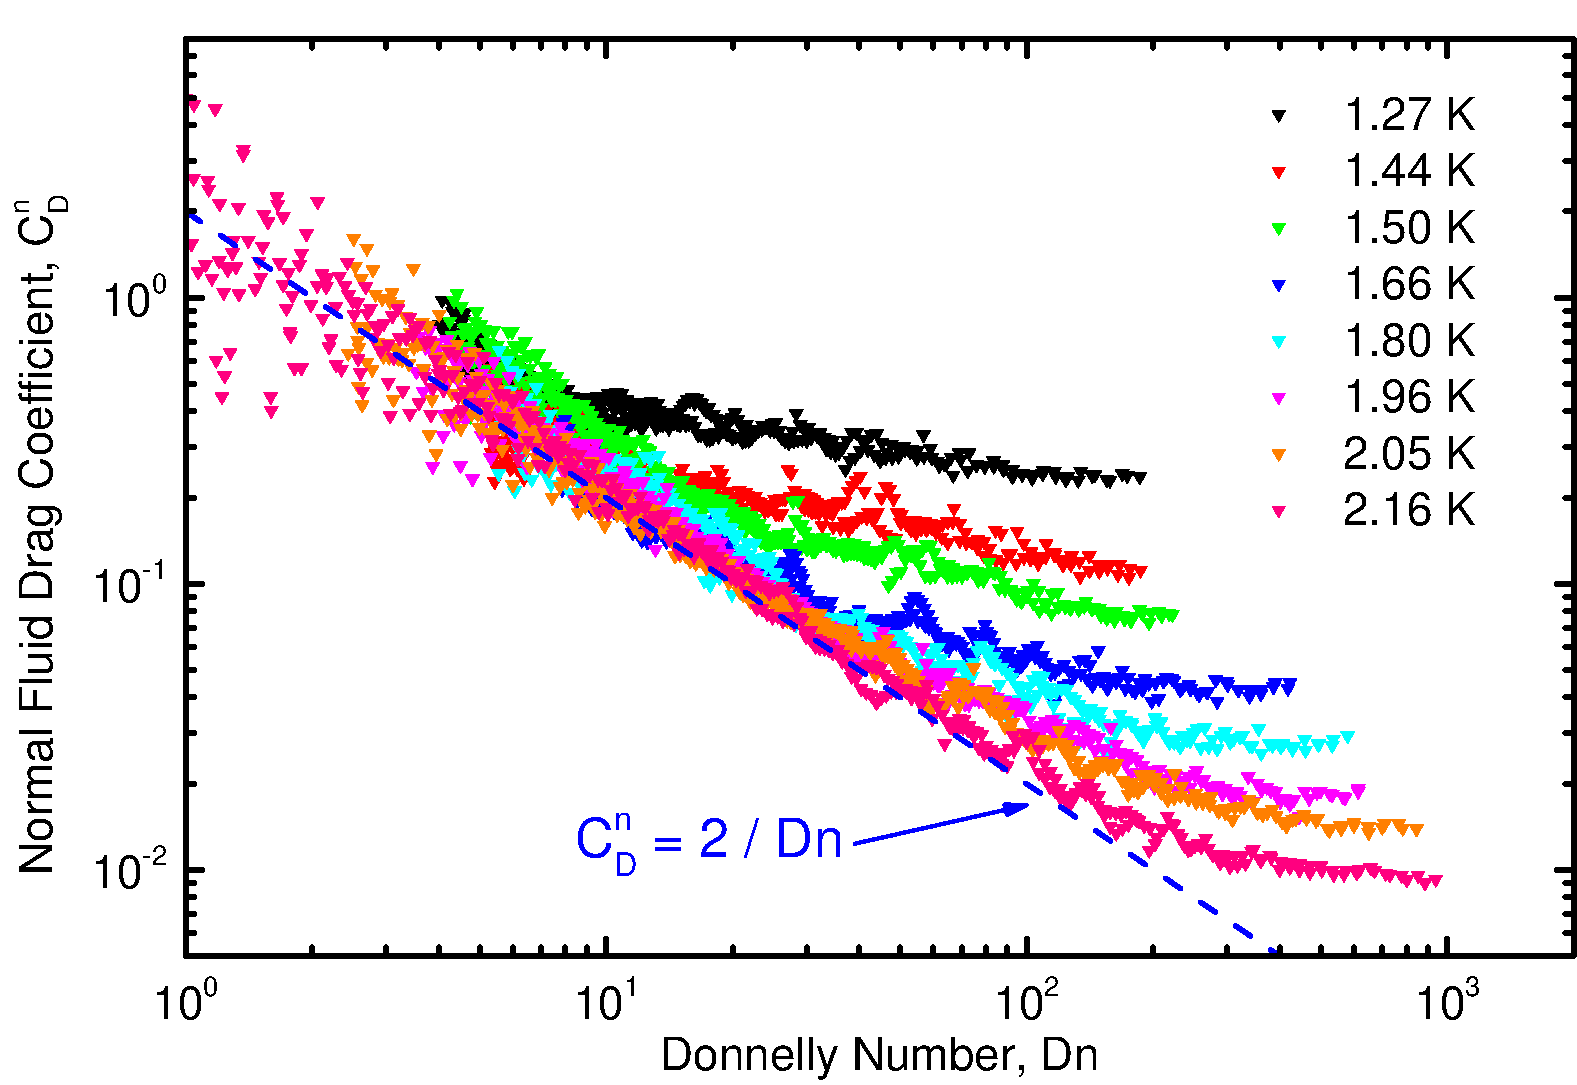
\includegraphics[width=0.7\textwidth]{graphics/results/disc_drag_donnelly}
  \caption{Plot of re-defined fluid drag coefficient $C_D^{\,n}$ against the dimensionless Donnelly number (Dn) for the torsionally oscillating disc at several temperatures.\\
  The \underline{blue dashed line} shows the expected theoretical dependence \cite{universal_scaling} for viscous drag. The temperature-dependent and temperature-ascending starting points of non-linearities are a clear sign of the onset of quantum turbulence by the superfluid component.}
  \label{disc_drag_donnelly}
\end{figure}


%%%%%%%%%%%%%%%%%%%%%%%%%%%%%%%%%%%%%%%%%%%%%%%%%%%%%%%%%%%%%%%%%%%%%%%%%%%%%%%%%%%%%%%%%%

\subsection{Tuning fork}

As the last oscillator, we used quartz tuning fork with geometry and resonant specifics as they were described in \textbf{Experimental approach} chapter. the resonant response was experimentally measured in the same way as was with vibrating wire - by a real-time analysis of the in-phase current and quadrature response. Electrical quantities are then converted into physical attributes according to mentioned relations (\ref{fork_conversions}), which are dependent on fork constants $a_{f0} = 3.665 \times 10^{-7} \unit{Cm}^{-1}$, $a_{f1} = 14.094 \times 10^{-7} \unit{Cm}^{-1}$ for the fundamental and overtone mode, respectively. \\
In order to measure the fork constants, we had to perform a series of frequency sweeps in low-temperature vacuum. We estimate the uncertainty of fork constants to be of $10\%$ since velocity calculation errors were proven using optical experiments. \cite{optical_exps}

\newpage

In \textbf{Figure \ref{fork-vel_force}} we plot the peak velocity response $U_0$ of the top of the fork prong, against the applied peak force $F_0$ at various temperatures from two-fluid regime ($T > 1.0\unit{K}$). We sketched the theoretical laminar $F_0 \propto U_0$ and classical turbulent dependencies $F_0 \propto U_0^2$ as guides for the eye.

\begin{figure}[h]
	% \centering
	\hspace{-1.7cm}
	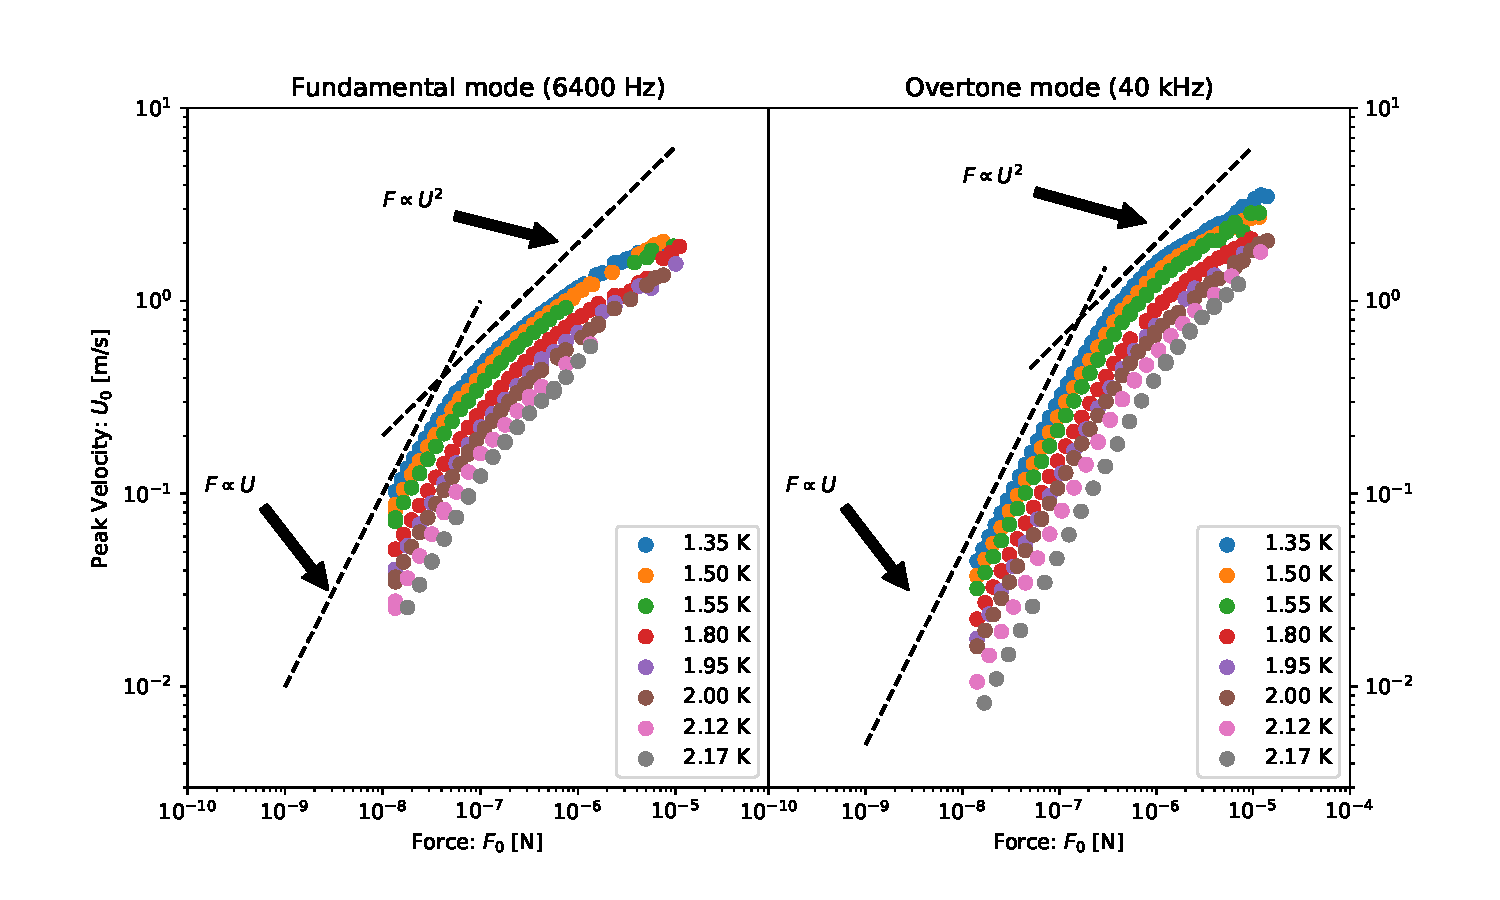
\includegraphics[width=1.2\textwidth]{graphics/results/fork-vel_force}
	\caption{Plot of peak velocity $U_0$ against the applied peak force $F_0$ for the oscillating tuning fork submerged in superfluid $\He$ at several temperatures.\\
	\underline{Left image:} Measurements in fork's fundamental mode, \underline{Right image:} Measurements in fork's overtone mode, \underline{Black dashed lines} mark the theoretical laminar and classical turbulent regime dependencies.}
	\label{fork-vel_force}
\end{figure}

We note that the linear sketched dependency decribe the laminar regime very well, whereas the quadratical (classical turbulence regime) seems to be a weak fit to the situation, especially for the lower temperatures from the studied range.

Next, we plot in \textbf{Figure \ref{fork-drag_vel}} the classical drag coefficient $C_D$ against the peak velocity $U_0$. Both oscillating modes are visualised as a paired plot in order to show their shared asymptote (as sketched with the black dashed line) in the area of big velocities. Also, we sketched the laminar regime fit as a demonstration.

\newpage

\begin{figure}[h]
	% \centering
	\hspace{-1.7cm}
	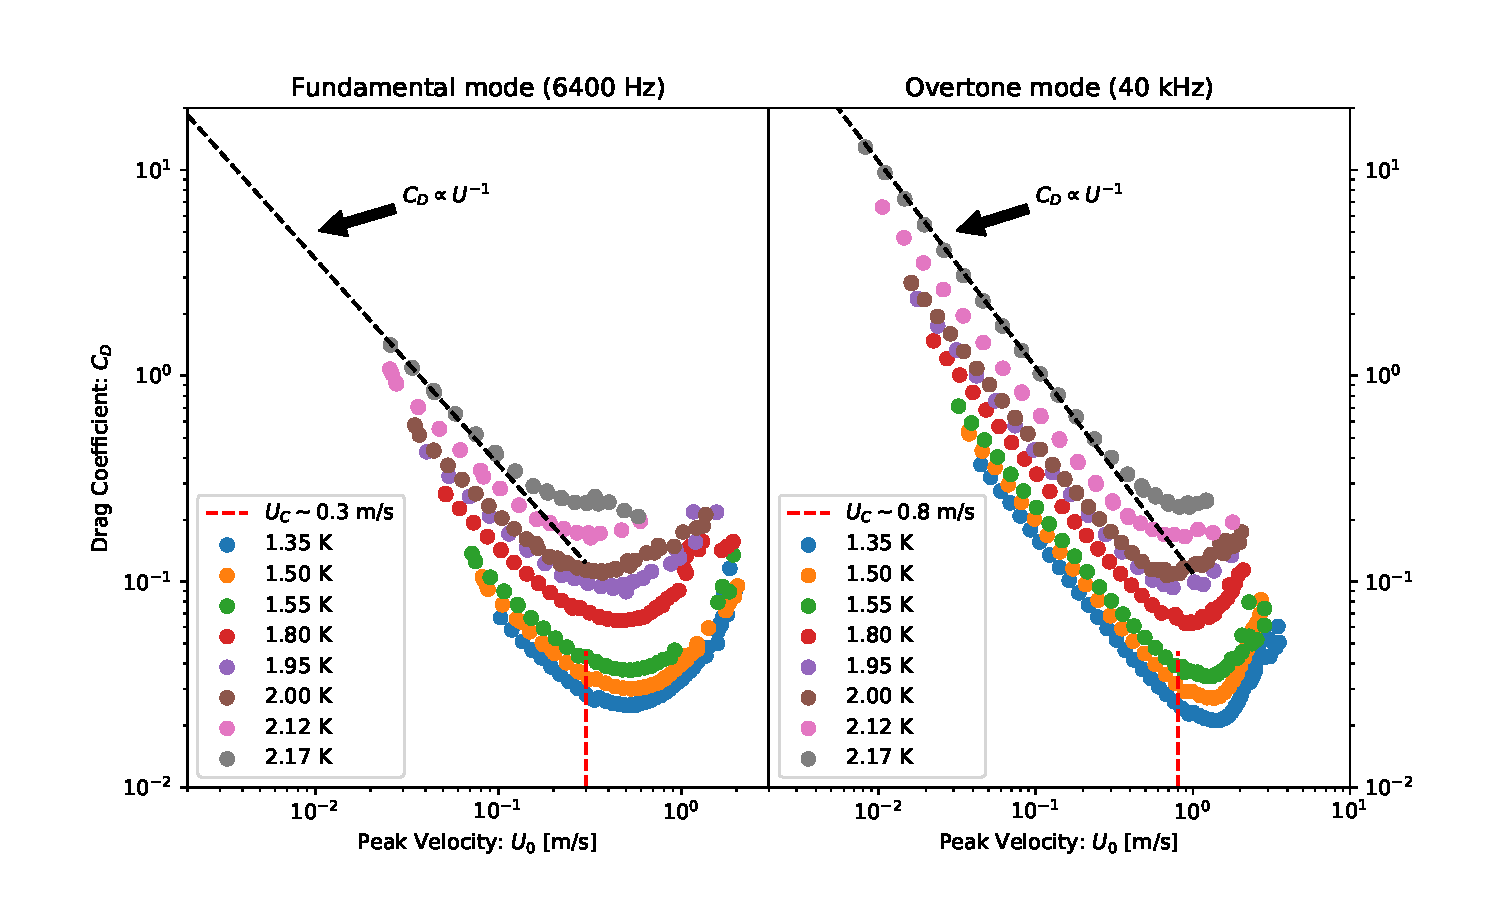
\includegraphics[width=1.2\textwidth]{graphics/results/fork-drag_vel}
	\caption{Plot of drag coefficient $C_D$ against the velocity peak response $U_0$ for the oscillating tuning fork submerged in superfluid $\He$ at several temperatures.\\
	\underline{Left image:} Measurements in fork's fundamental mode, \underline{Right image:} Measurements in fork's overtone mode, \underline{black dashed line} fits the theoretical laminar regime dependency, \underline{red dashed line} marks the critical velocity value $U_C$ above which an onset of quantum turbulence appears. The clear sign of this effect can be seen for a group of curves with $T < 1.6\unit{K}$.}
	\label{fork-drag_vel}
\end{figure}

As expected, the tuning fork exhibits a linear drag in the area of low velocities regardless on the temperature from the studied range. Then, approximately above the critical velocity $U_C$, a synchronized increased drag was observed for a group of curves with temperature $T < 1.6\unit{K}$, which is a clear sign of onset of quantum turbulence. The critical velocities differ for oscillating modes:

\begin{equation}
U_{C0} \sim 0.3 \unit {m/s}
\hspace{1cm}
U_{C1} \sim 0.8 \unit {m/s}\,,
\end{equation}

which is expected from the scaling relation (\ref{drag_super}) and roughly proven since the critical dimensionless velocities $\hat{U}_{C0} = U_{C0} / \sqrt{ \varkappa \omega_0} \approx 4.7$ and $\hat{U}_{C1} = U_{C1} / \sqrt{ \varkappa \omega_1} \approx 5.0$ are similar.

Curves with higher temperature seem to transit to non-linear regime earlier, which indicates the classical turbulence of the normal component instead.

\newpage

To characterize the normal component flow, we plot in \textbf{Figure \ref{fork-drag_donnelly}} the normal drag coefficient against the dimensionless Donnelly number. The conversions were done as we stated in (\ref{universal_scale}).

\begin{figure}[h]
	% \centering
	\hspace{-1.7cm}
	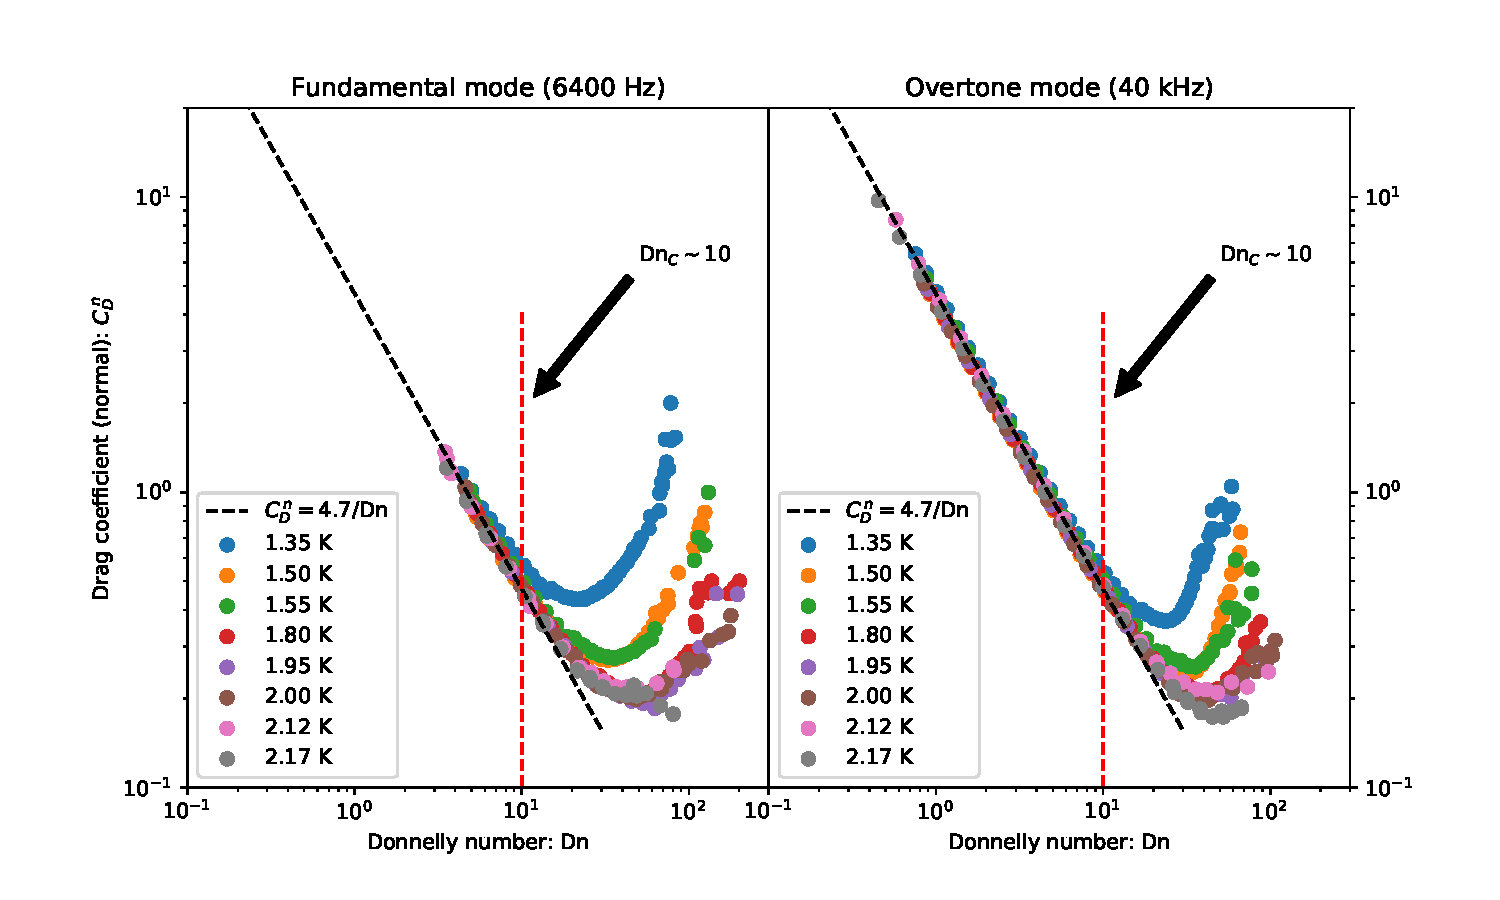
\includegraphics[width=1.2\textwidth]{graphics/results/fork-drag_donnelly}
	\caption{Normal fluid drag coefficient $C_D^{\,n}$ as a function of the Donnelly number Dn. \underline{Left image:} Measurements in fork's fundamental mode, \underline{Right image:} Measurements in fork's overtone mode, \underline{Black dashed line} fits the theoretical laminar regime dependency, with the same pre-factor $C_D^{\,n} = 4.7 / \text{Dn}$ for both oscillation modes, \underline{Red dashed line:} the estimated critical value of Dn, above which the onset of classical turbulence occurs for the group of temperature curves $T > 1.6 \unit{K}$.}
	\label{fork-drag_donnelly}
\end{figure}

With no doubt, in the area of low Donnelly values, the dependencies collapse to a single line as expected, representing the laminar regime with the shared pre-factor $\Phi \sim 4.7$. In contrast to the results obtained with the vibrating wire or oscillating disc, we also recognize, additionally to the critical velocity $\hat{U}_C$, a critical value of Donnelly number $\text{Dn}_C$, above which the rest group of temperature curves $T > 1.6\unit{K}$ non-linearly deviate.
The onset of turbulence for these curves is governed by a single value of Donnelly number $\text{Dn}_C$ and thus dominated by the classical turbulence of the normal component.\\
We note that it is interesting to find the laminar pre-factor $\Phi \sim 4.7$ to be same for both oscillation modes. The shared critical $\text{Dn}_C$ was expected from the dynamical similarity principle, but the shared $\Phi$ is a result of different principle - the fact that both modes have the same effective mass $m_{\text{eff}}$ (see \cite{universal_scaling}).

\newpage

We found the approximate value for the shared critical Donnelly number $\text{Dn}_C$ again using \textit{error plot}, where the \textit{error} is here defined via the normalized deviation rate from the laminar fit $f: C_D^{\,n} \text{Dn} - \Phi$, where $\Phi = 4.7$ as:

\begin{equation}
\text{Error} = \frac{\text{abs}(C_D^{\,n} \text{Dn} - \Phi)}{C_D^{\,n}\text{Dn}} \in (0,1)
\end{equation}

We plot these errors in \textbf{Figure \ref{fork-error_donnelly}} in order to mark more clearly the position of $\text{Dn}_C$, where the group of temperatures $T > 1.6\unit{K}$ starts to deviate.

\begin{figure}[h]
	% \centering
	\hspace{-1.7cm}
	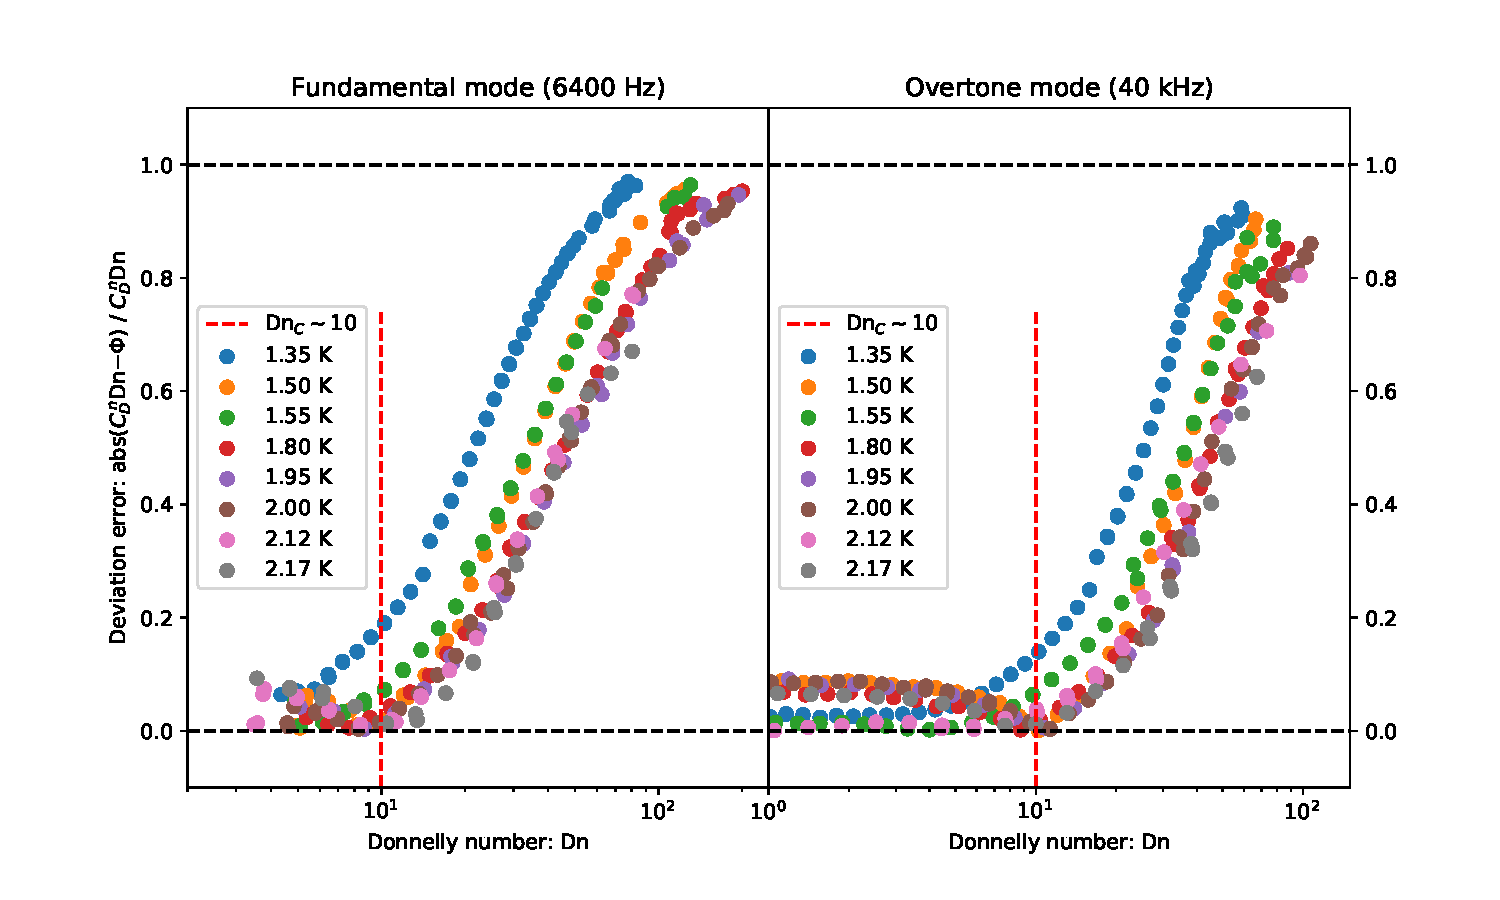
\includegraphics[width=1.2\textwidth]{graphics/results/fork-error_donnelly}
	\caption{Plot of normalized deviations from the linear fit $C_D^{\,n} =  \Phi / \text{Dn}$ with $\Phi = 4.7$ as a function of the Donnelly number. \underline{Left image:} Errors in fork's fundamental mode, \underline{Right image:} Errors in fork's overtone mode, \underline{Black dashed lines} mark the boundaries and \underline{red dashed lines} our estimations for the values of Dn${}_C$.
	}
	\label{fork-error_donnelly}
\end{figure}

Our estimated value for critical Donnelly number $\text{Dn}_C$ for temperature curves $T > 1.6\unit{K}$ and for both oscillation modes is $\text{Dn}_C \sim 10$. This shared value of $\text{Dn}_C$ proves the high-frequency regime validity and thus the possible domination of classical turbulence from normal component.

\section{Ballistic regime}

In this section, we demonstrate the limits of universal scaling validity. In \textbf{Figure \ref{ballistic}} we plot the scaling function of Weissenberg number $f(\text{Wi})$, as derived in \cite{scaling_function} and introduced in the \textbf{Theoretical Background} in (\ref{scaling_function}). In order to validate the derivation, we add the experimental results obtained with a tuning fork in two-fluid regime (presented in previous section) and also in ballistic regime ($T < 0.6\unit{K}$).
Again, these regimes represent the Newtonian hydrodynamics ($\text{Wi} \ll 1$), governed by Navier-Stokes equations, and a non-newtonian gas dynamics. \cite{universal_scaling}

\begin{figure}[h]
	\centering
	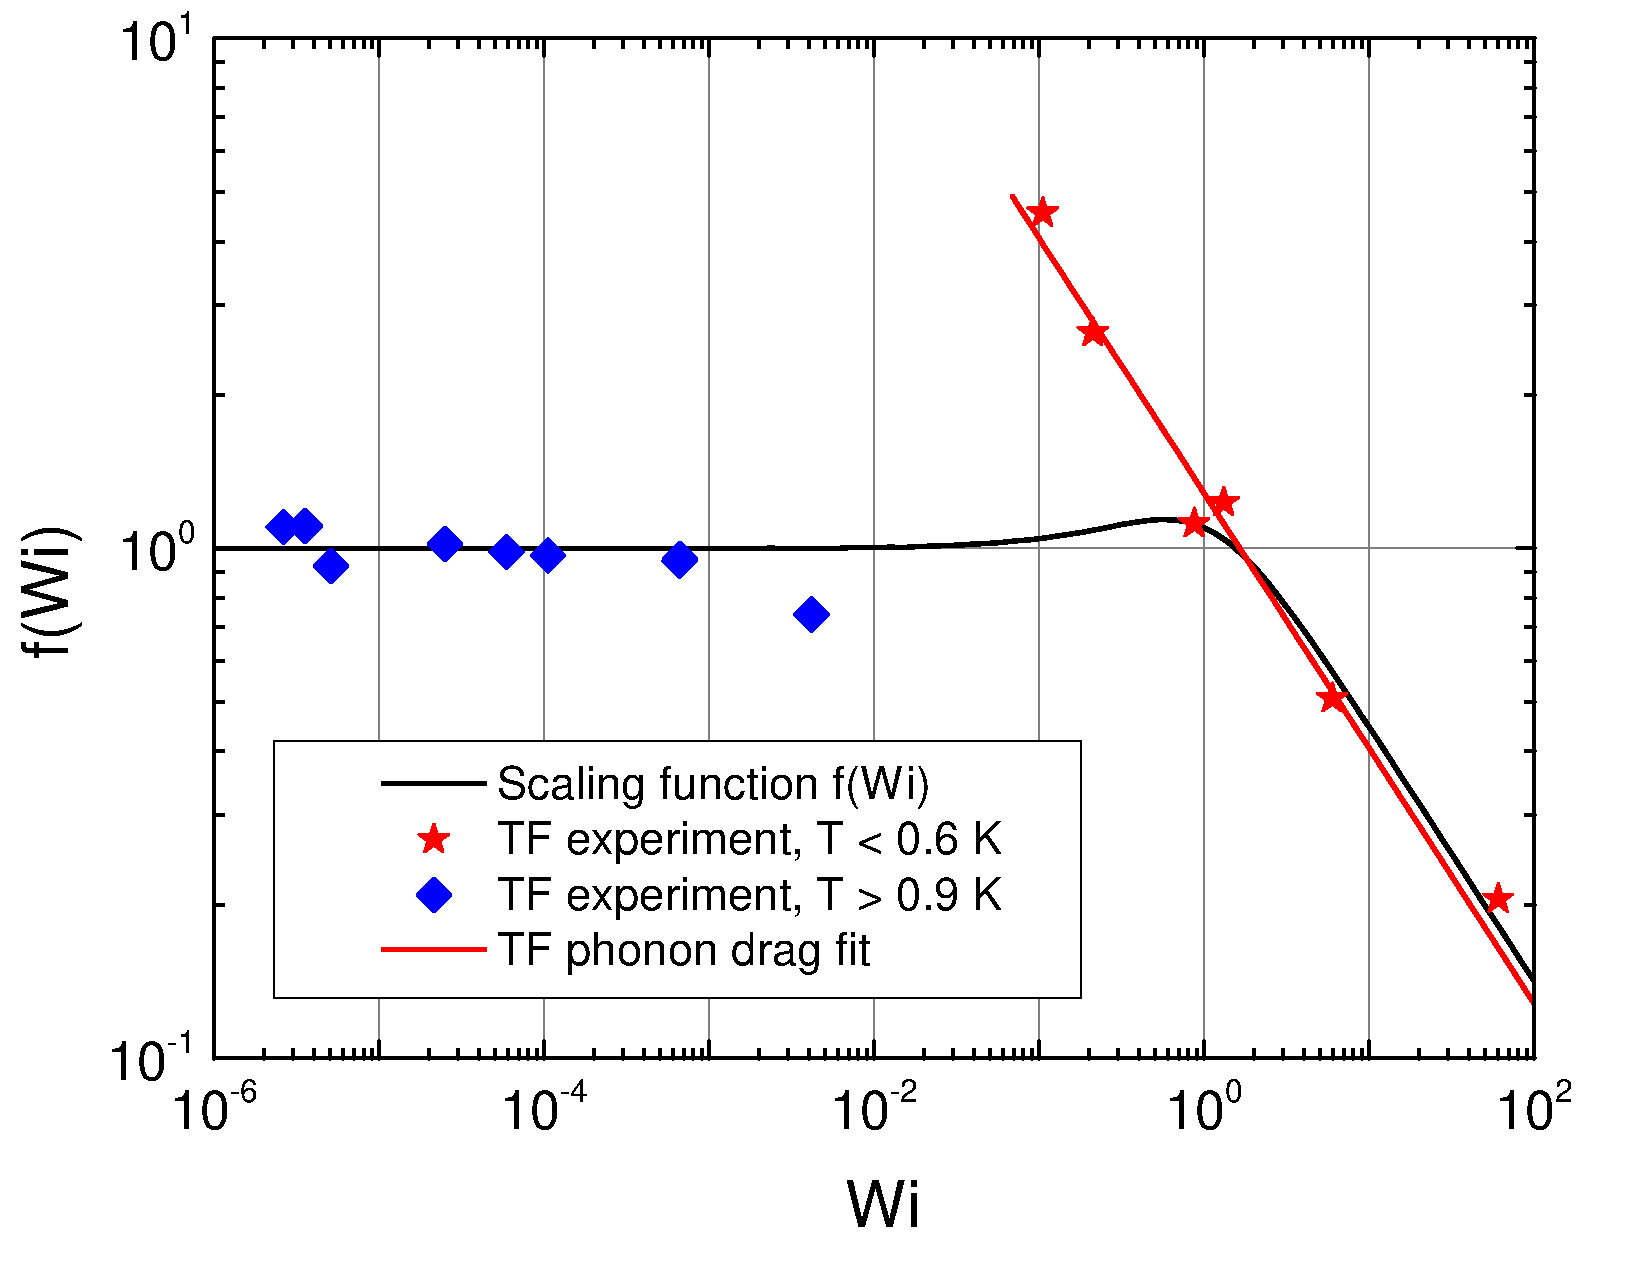
\includegraphics[width=0.7\textwidth]{graphics/results/ballistic_regime}
	\caption{Plot of scaling function $f(\text{Wi})$ as proposed in (\ref{scaling_function}) compared with the experimental results of tuning fork in both low and ultra-low temperatures.\\
	\underline{Black line:} fit of the scaling function, \underline{Red line:} fit to the phonon drag \cite{universal_scaling} , \underline{Blue squares:} experimental data collected from mentioned experiments, \underline{Red stars:} experimental data collected from ultra-low temperature range. In all experiments we used the same tuning fork on both oscillation modes.}
	\label{ballistic}
\end{figure}

Both asymptotics for $\text{Wi} \rightarrow 0$ and $\text{Wi} \rightarrow \infty$ are identical in the means of quasi-classical description of the excitation gas.
The mean free paths (or relaxation times) therefore can be calculated quantum-mechanically.\\
The derived behaviour of scaling function ($f(\text{Wi}) \sim 1$ for $\text{Wi} \ll 1$ and $f(\text{Wi}) \propto 1/\sqrt{\text{Wi}}$ for $\text{Wi} \gg 1$) reflects the experimental data, except for the transitional area $\text{Wi} \sim 0.1 $, where emerged a bigger peak than expected.\\
However, according to \textbf{Figure \ref{Kn-Wi}}, this is the range where the fluid have already reached the ballistic regime ($\text{Kn} \sim 1$) earlier than the non-Newtonian one ($\text{Wi} \sim 1$).
Hence, the assumptions for the scaling function derivation (that both $\text{Kn, Wi} \sim 1$) are no more valid and thus our prediction $f(\text{Wi}) \propto 1$ for the problematic area $\text{Wi} \sim 0.1$ does not hold.\\
In this case, the apparent scaling $f(\text{Wi}) \propto 1/\sqrt{\text{Wi}}$ simply means a frequency-independent drag force, as is expected for the ballistic regime.

\section{Flow phase diagram}

The last plot we show in \textbf{Experimental results} is the \textit{flow phase diagram}, summarizing the achieved hydrodynamical states by the oscillating tuning fork at various temperatures and modes. In \textbf{Figure (\ref{fork-flow_phase})} we also mark the estimated areas ("CT" for classical turbulence and "QT" for quantum turbulence), where the transitions to non-linear regimes emerge, separately for the normal and superfluid component.

\begin{figure}[h]
	\centering
	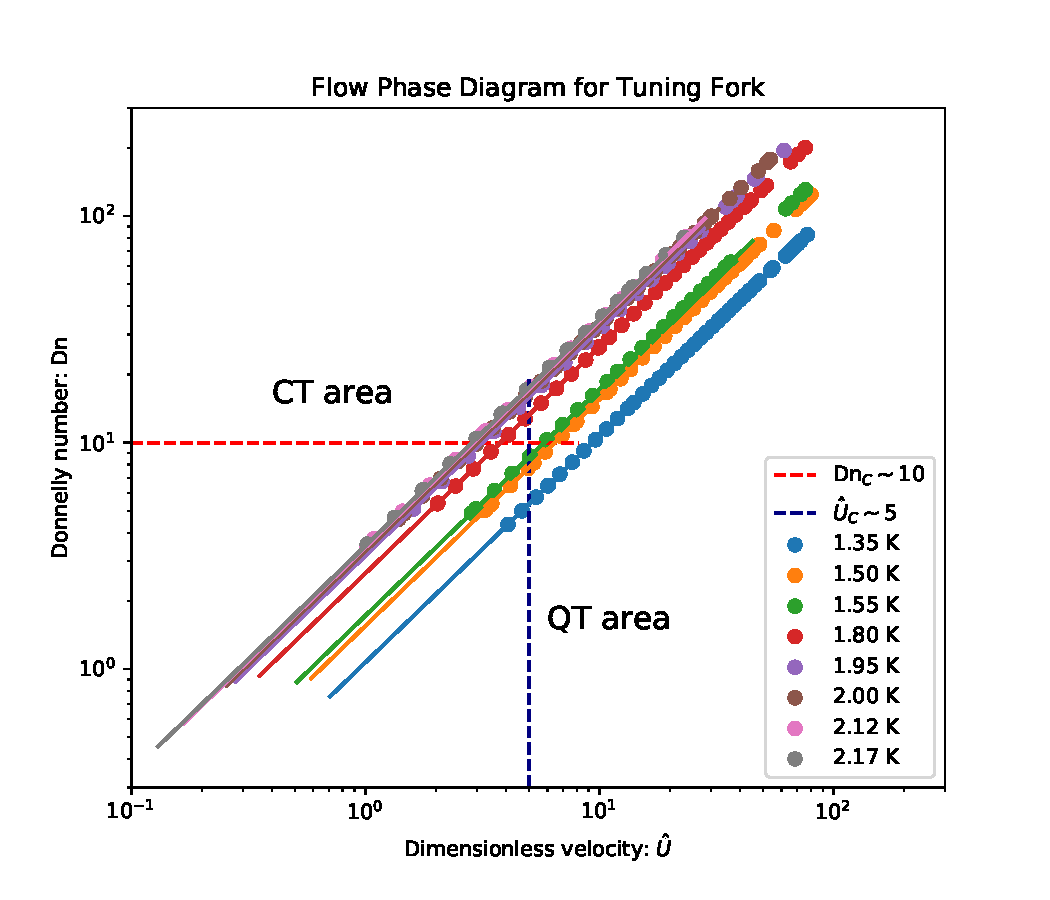
\includegraphics[width=0.8\textwidth]{graphics/results/fork-phase}
	\caption{Plot of Donnelly numbers against dimensionless velocities for both fork's oscillation modes. \underline{Full lines} fit the overtone mode data and \underline{dashed lines} the estimated areas of transition from laminar/potential regimes to the non-linear ones, both for normal and superfluid components.}
	\label{fork-flow_phase}
\end{figure}

It is worth to note that the \textit{CT area} and \textit{QT area} are not so sharp as it may seem from the graph. First of all, the most of the graph is covered by \textit{mixed turbulence} area since we already hinted that QT probably directly triggers CT.\\
Also, there could not be any more data above the $T=2.17\unit{K}$ curve since it is the natural limitation for the warmest Helium-II system.
